\chapter{Detección de objetos} 
Uno de los objetivos del desarrollo de este proyecto es procesar la imagen capturada por una cámara RGB que forma parte de la estructura de un robot de servicio industrial, cuya tarea es manipular objetos entre estaciones de trabajo, buscando mejorar su desempeño utilizando la información obtenida . En pos de esto, se realizó el siguiente desarrollo.

\section{Objetos de interés}
Los objetos que se busca identificar tienen características muy específicas y son fácilmente identificables dentro del espacio de trabajo del robot. Este fue uno de los motivos por los que el procedimiento actual fue propuesto. Se trata de las \textbf{bases}, cilindros huecos de colores sólidos (negro o rojo), así como de \textbf{anillos} que es posible apilar sobre dichos cilindros y entre ellos, a manera de piezas intermedias, estos pueden ser amarillos, verdes o azules. Tanto las bases como los anillos tienen $4.5\times4.5 [cm]$ de diámetro. 
El objetivo de esta etapa es identificar dichos objetos dentro de las imágenes obtenidas por la cámara del robot y asignarles una coordenada cartesiana asociada al mapa que el robot utiliza como referencia.
Estas piezas destacan por su color, dado que los demás elementos en el espacio de trabajo del robot tienen colores predominantemente azules o grises.
 
\begin{figure}[ht]
\centering
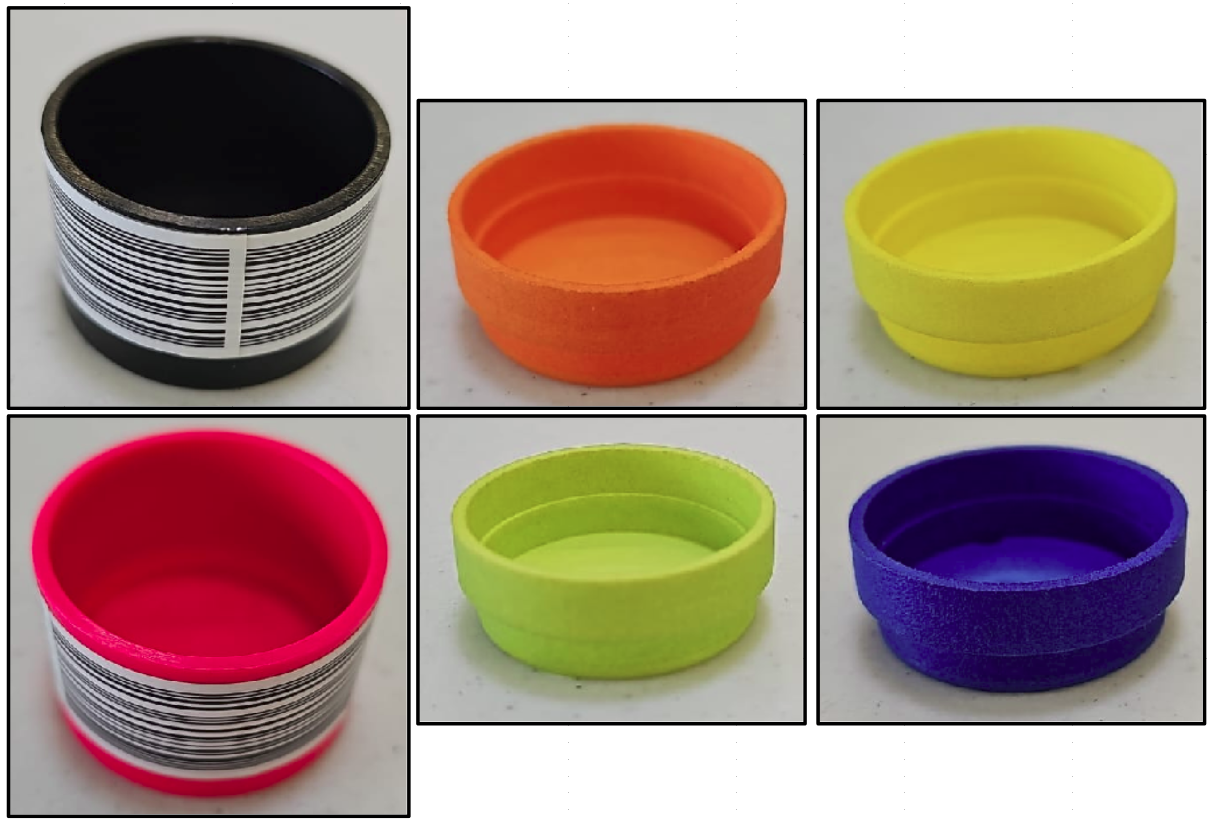
\includegraphics[scale= 0.15]{Figures/Pieces.png}
    \caption{Objetos de Interés}
    \label{fig:Pieces}
\end{figure}

Como se puede observar en la figura \ref{fig:Pieces} las diferencias de color entre las piezas son claras, por lo que es posible diferenciarlas entre sí utilizando como herramienta la segmentación por color. Además, dentro del espacio de trabajo (ver figura \ref{fig:EspaciodeTrabajo}) del robot, las piezas pueden encontrarse un área muy reducida dentro de la cual es muy poco probable que se encuentre algún elemento con características de color similares.

\begin{figure}[H]
\centering
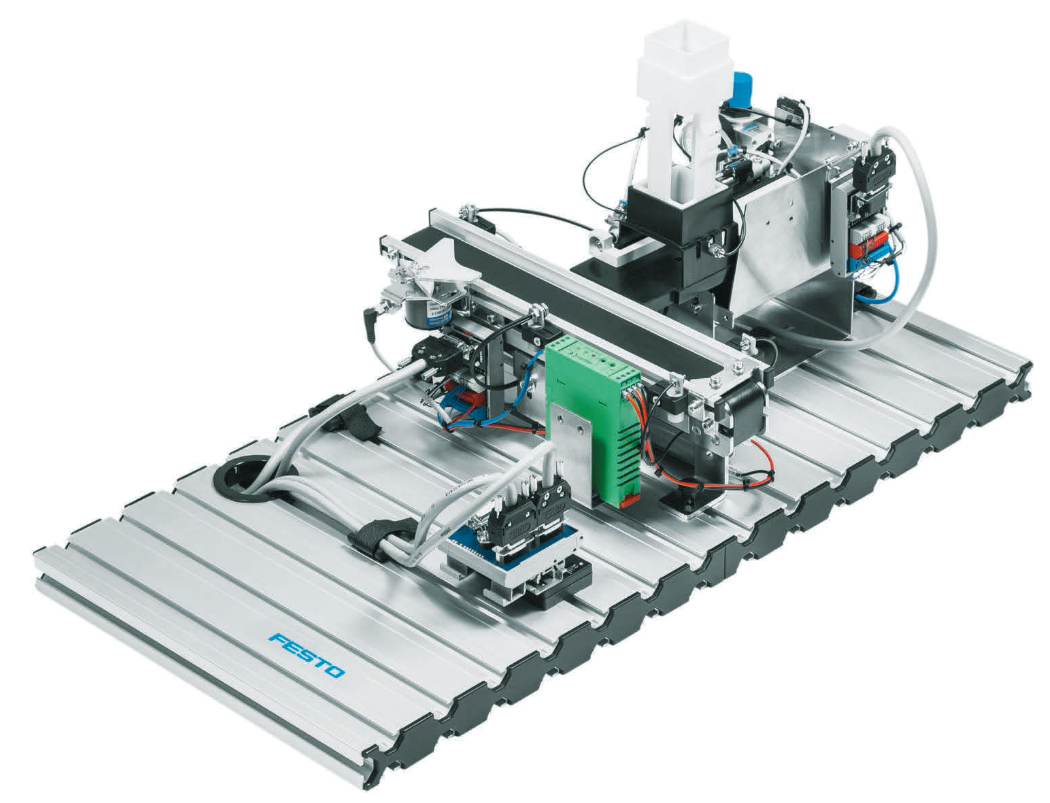
\includegraphics[scale= 0.2]{Figures/BandaTrans_Big.png}
    \caption{Ejemplo del espacio de trabajo del robot}
    \label{fig:EspaciodeTrabajo}
\end{figure}

Adicionalmente, la región de interés dentro del espacio de trabajo es bastante reducida, dado que el procesamiento de las piezas se lleva dentro de la s estaciones de forma independiente al comportamiento del robot, por lo que se cuenta con dos regiones importantes dentro del espacio de trabajo sobre las estaciones, que corresponden a la entrada y la salida de la banda transportadora, de donde el robot debe tomar la pieza para ser procesada y, una vez que la estación de trabajo ha concluido su tarea, debe recoger la pieza de la salida de la banda transportadora para llevarla al siguiente paso en la secuencia de ensamblado.

\section{Caracterización de los objetos}
El primer paso dentro del procedimiento fue capturar imágenes de los objetos bajo diferentes condiciones de luz. Dada la curvatura de la superficie de los objetos, así como la regiones que en el interior de los cilindros, se obtenían variaciones de color debidas a las sombras, por este motivo, se tomó la media de color no solo con cambios de iluminación sino también considerando diferentes regiones de las piezas.

\begin{figure}[H]
\centering
\includegraphics[scale= 0.35]{Figures/Tabla_Iluminación.png}
    \caption{Efectos de los cambios de Iluminación en las piezas}
    \label{fig:Ilumination}
\end{figure}

Con las imágenes de referencia obtenidas en el espacio de color RGB se realizó la conversión al espacio HSV, en el cual se llevó a cabo la obtención de los vectores correspondientes a las medias de color en este espacio.

\begin{figure}[H]
\centering
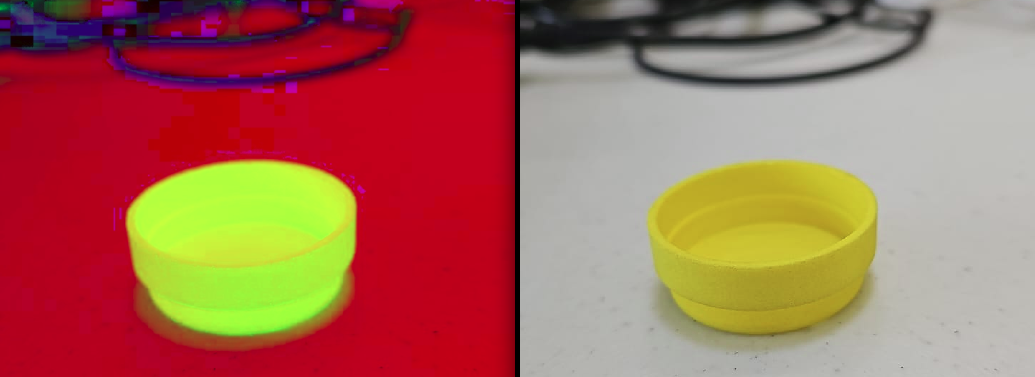
\includegraphics[scale= 0.3]{Figures/HSV_YellowRing.png}
    \caption{Ejemplo de Anillo amarillo en: izq) HSV} y der) RGB
    \label{fig:YellowRing_HSV}
\end{figure}

\textcolor{yellow}{Agregar figura del mismo objeto con diferentes iluminaciones. De ser posible hacer una tablita. Columna izquierda, imágenes pequeñas con diferentes iluminaciones y en la derecha la media de color}

\begin{figure}[H]
\centering
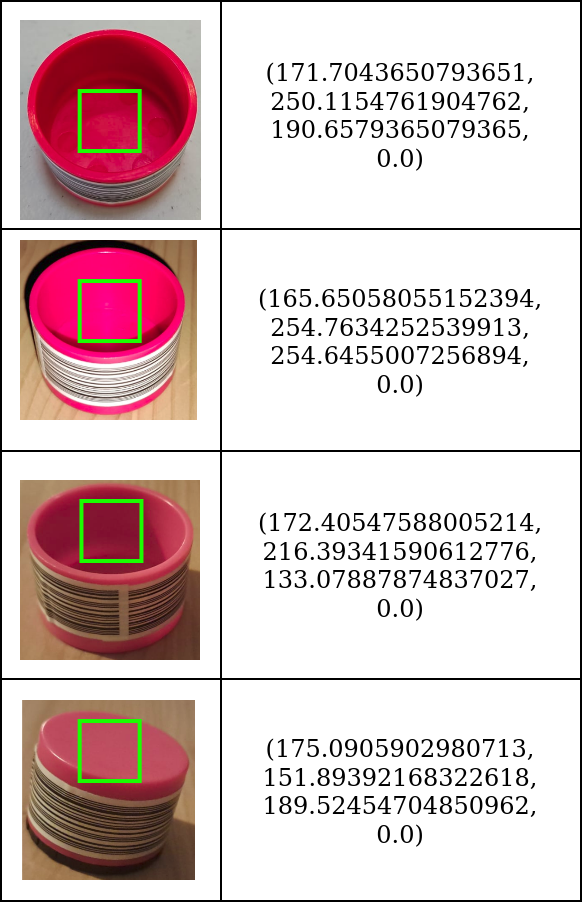
\includegraphics[scale= 0.3]{Figures/Tabla_Medias_Ilum.png}
    \caption{Medias de color a diferentes iluminaciones y en diferentes regiones - Base roja}
    \label{fig:RedPiece_MeanHSV}
\end{figure}

Una vez que se tiene esta información se pasó a la umbralización de las imágenes a evaluar (en este caso el vídeo proporcionado por la cámara KINECT). De esta forma, cada cuadro que compone al vídeo se convierte al espacio HSV y se filtran aquellos píxeles que corresponden con la media de color de las imágenes de referencia. 

\begin{figure}[H]
\centering
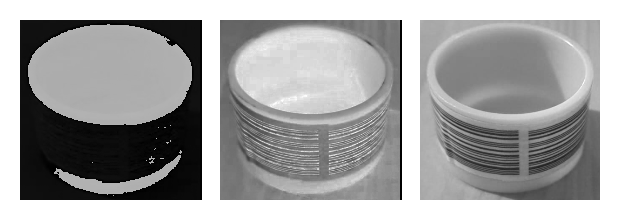
\includegraphics[scale= 0.3]{Figures/RedPiece_HSV_components.png}
    \caption{Pieza Roja - Componentes a) H b) S c) V}
    \label{fig:RedPiece_HSV}
\end{figure}


Para este filtrado fue necesario establecer los umbrales superior e inferior dentro de los cuales se considera que se cumplen las condiciones de la media de color. Estos umbrales permiten asignar una cierta tolerancia para los píxeles que por cambios de iluminación no correspondan exactamente con la media buscada. Para considerar estos cambios se realizó el proceso de umbralización considerando diferentes medias de color, obteniendo entonces varias máscaras que representaban al objeto dependiendo de las secciones del mismo cuyas medias de color coincidían. Finalmente, se aplicó la operación lógica OR entre las máscaras obtenidas, resultando en una máscara compuesta por todos los píxeles que coincidían con todas las variaciones de iluminación considerados.

\begin{figure}[H]
\centering
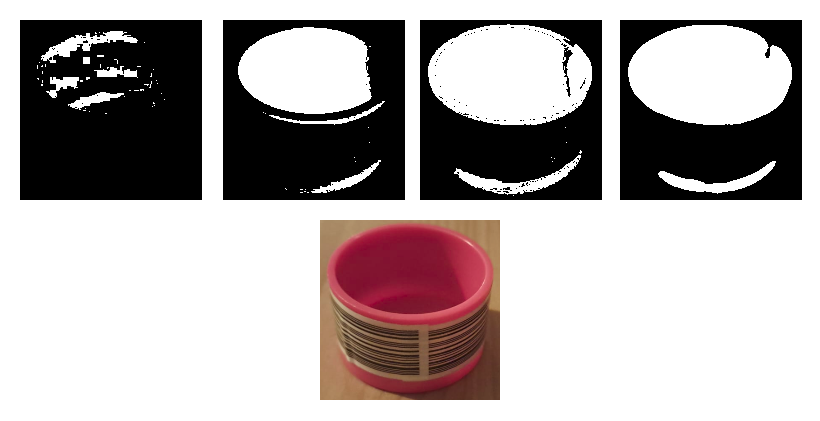
\includegraphics[scale= 0.35]{Figures/Masks_Piece.png}
    \caption{Pieza Roja}
    \label{fig:Masks_RedPiece}
\end{figure}

En la figura \ref{fig:Masks_RedPiece} se pueden observar las distintas máscaras correspondientes a las medias de color mostradas en la figura \ref{fig:RedPiece_MeanHSV}. La última máscara, a la derecha de la imagen, corresponde a la combinación de todas las anteriores. En esta figura se observa el comportamiento del algoritmo con una imagen de la pieza aislada, mientras que en la figura \ref{fig:Masks_WorkSpace} se puede apreciar el efecto del algoritmo en una imagen de la pieza dentro del espacio de trabajo estándar que el robot de servicio habría de encontrar en condiciones reales. En este proceso, además, se agregan las operaciones \textit{erosión} y \textit{dilatación}, la primera utilizada para reducir el ruido obtenido del filtrado por elementos en el espacio de trabajo que estén dentro del rango de color solicitado. Como se puede observar, existen grupos de píxeles en la imagen que desaparecen con la operación erosión al ser demasiado pequeños para considerarse como un elemento de interés. Finalmente se aplica la operación dilatación para recuperar los píxeles  de los bordes del objeto que se hayan reducido durante la erosión. 

\begin{figure}[H]
\centering
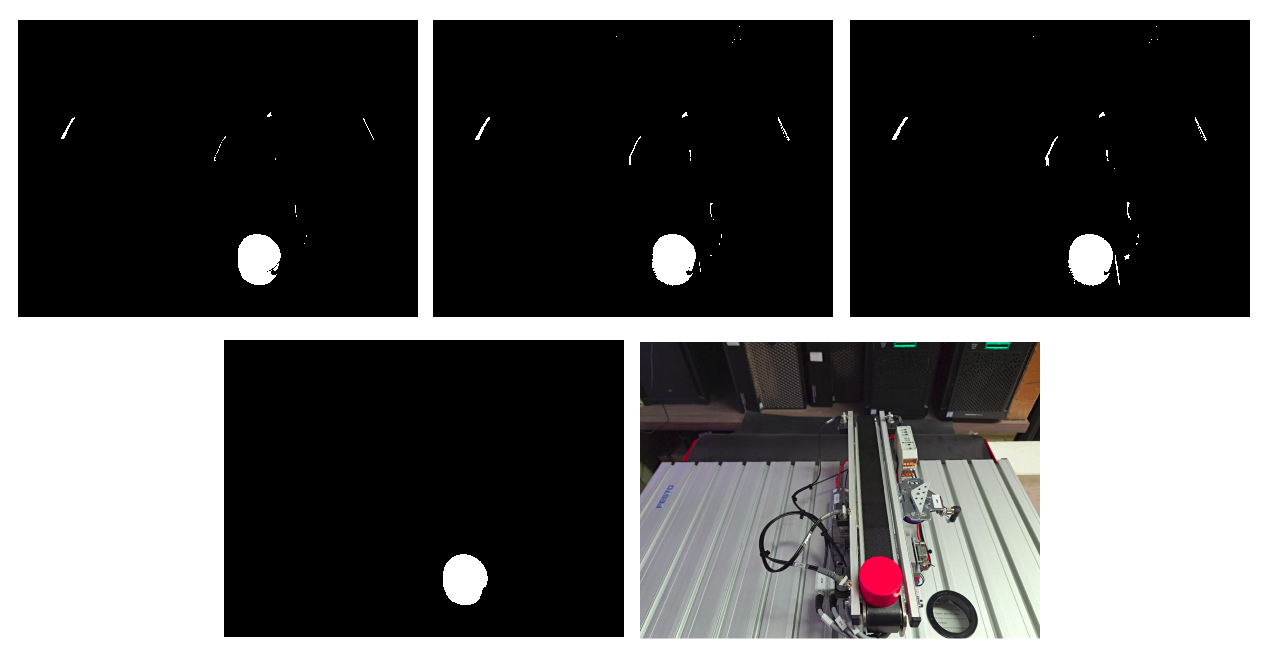
\includegraphics[width=\textwidth]{Figures/Masks_WS_3.png}
    \caption{Espacio de Trabajo}
    \label{fig:Masks_WorkSpace}
\end{figure}

\section{Localización de objetos}

Una vez obtenida la máscara que contiene todos los píxeles que coinciden con el modelo del objeto de interés se realiza la localización del objeto en el espacio tridimensional. Ya que se ha aislado la pieza en la imagen se obtiene el centroide geométrico del conjunto de píxeles en blanco, representando el centro de la pieza. 


\subsection{Nubes de puntos}

Para la obtención de la nube de puntos se utilizó el sensor de profundidad incluido en el dispositivo Kinect, este sensor emite un pulso de luz infrarroja y mide el tiempo que toma el pulso desde que es emitido hasta que regresa al sensor después de haber rebotado en una superficie, con este tiempo el dispositivo calcula la distancia estimada desde el sensor hasta el objeto, de acuerdo con la información del fabricante, el sensor utilizado para este proyecto cuenta con una resolución de $640 \times 480$ píxeles \cite{davison_kinect_2012}. Este conjunto de medidas de profundidad se asocian con su posición respecto al sensor, dando lugar a un \textit{mapa de profundidades}. Para la estimación de la posición del objeto en el espacio, se realiza la comparación entre la imagen obtenida por la cámara RGB y el mapa de profundidades, asociando el centroide obtenido del objeto de interés con la información de la distancia calculada por el sensor de profundidad, resultando en la posición de la pieza en coordenadas relativas al dispositivo Kinect.
